% Background Information

\chapter{The Algorithm} % Main chapter title

\label{chap:Algorithm} % For referencing the chapter elsewhere, use \ref{Algorithm} 


%----------------------------------------------------------------------------------------
\section{Approach}
The algorithm can be divided in a number of parts that will be discussed during the coming sections. These steps need to be taken in order to complete the process of converting a $CFG$ to a syntax highlighter. This algorithm was build with Sublime Text in mind, however it is easy to make extensions or modifications to it in order to make it work for other editors.\\
The idea is to convert the grammar to its regular approximation using the algorithm presented in \cite{MohriNederhof}. Then turn this approximation into the corresponding state machines. With these machines, the states can then be mapped to contexts and from those a highlighter is created. A few things to consider here are:
\begin{enumerate}
\item How to preserve highlighting information found in the original $CFG$?
\item Do the transformations cause information loss that is essential for correct highlighting?
\item Does the final result do a good (enough) job at highlighting?
\end{enumerate}

\section{The Algorithm's Pipeline} \label{sec:Pipeline}
For embedding highlighting information this algorithm needs information per token in the right-hand side of a production rule. This is a specification of the scope to use for highlighting these tokens. This allows for the same non-terminals being coloured differently depending on the context (Think of identifiers as function names or as simple variable names in \textit{Java} or \textit{C}, the first is blue and one is white). Below is a simple example of what a rule could look like. Indicating that all elements on the right-hand side should be coloured with the named scope. The specification could either be a list of scopes, a single scope, or no scope(s) at all.
\begin{equation*}\prodgr{String}{@Context="string.quoted.double" \hspace{.2in}"\hspace{.1in} StringChar \hspace{.1in}"}\end{equation*}\\\\\\\\\\\\\\\\\\
Any form that indicates information about the tokens on the right-hand side of a rule will be sufficient. For this project the above notation will be used with the following rules:
\begin{enumerate}
\item The $"@Context"$ tag is followed by a space-separated list of scopes enclosed by a pair of double quotes. There is one scope for each token on the right hand side. 
\item If no context is specified, no tokens will be coloured.
\item The token $null$ means no colouring.
\item If there are less than $N$ scopes specified, where $N$ is the number of tokens on the right-hand side, then the last scope in the list will be used for the remaining items.
\end{enumerate}
 
 	\subsection{Example grammar}
 	The upcoming sections describe the different steps to take in the algorithm. For illustrative purposes the following grammar will be used. This is a plain context-free grammar and these steps will for now be untailored to specific programming languages.
\begin{lstlisting}[language=RascalGrammar]
start Statement	->	Id ":=" Literal
					->	@@Context="keyword.control.flow null">@ 
							"if" "(" Condition ")" "{" Statement "}"

Condition	->	Id ">" Id
			 		->	Id "<" Id
					->	Id "==" Id

Literal		-> String
					-> Integer

Integer		-> @@Context="constant.numeric.integer">@ [0-9]+
Id				-> [a-z]+
String		-> @@Context="string.quoted.double">@ "\"" ![\"]* "\""
\end{lstlisting}

	\subsection{Simplifying the grammar}
	The first step is to reduce any grammar formalism used to the standard 4-element tuple as defined in \ref{sec:CFG_def}. Most programming languages do not have such a clean implementation of context-free grammars. In order to make any implementation work it is essential to convert the input grammar to the default form. Do make sure to keep the information about the scopes. What to do here is different per programming language. How this works for Rascal will be discussed in the chapter on implementation (\ref{chap:Implementation}).
	\pagebreak
	
	\subsection{Grammar to Graph}
	After the grammar is clean, compute the graph of the grammar implementing the method described in \ref{eqn:gram2graph}. Since the grammar is reduced to $(V, \Sigma, P, S)$ it is a simple loop over all elements of $P$ to compute this.
	\subsubsection{Example}
	\begin{figure}[H]
		\centering
		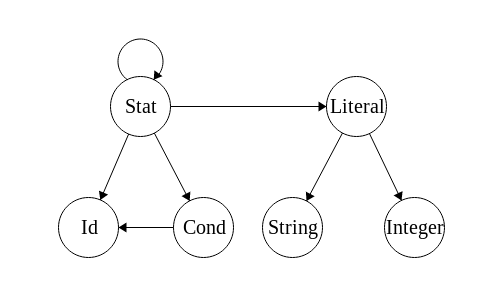
\includegraphics[scale=0.6, keepaspectratio]{Figures/grammarGraphChap2.png}
		\decoRule
	 	\caption[Graph of the example grammar]{The constructed graph of the grammar}
	 	\label{fig:chap2:graphOfExample}
	\end{figure}
	
	\subsection{$CFG$ to Strongly Regular Grammar}
	To make this conversion use the algorithm described in \ref{sec:MohriNederhof}. First take the graph obtained from the previous step and compute its strongly connected components using Kosaraju's algorithm (\ref{sec:Kosaraju}). These components correspond to the mutually recursive sets of symbols that Mohri's algorithm uses. Since the new symbols that are introduced by the transformation correspond to the ending of the original symbols, $A'$ can be viewed as something like $A_{end}$.
	\subsubsection{Example}
	The strongly connected components of the graph is the same as the graph itself since it contains no cycles. Only the self loop of \textit{Statement} would be gone. Therefore it is not included again. The strongly regular version of this grammar is shown below. There is only one component in violation of the either all left- or right-linear production rules. These are the rules of Statement. An extra non-terminal is introduced and the transformation is performed.
\begin{lstlisting}[language=RascalGrammar]
start Statement	->	Id ":=" Literal Statement_end
								->	"if" "(" Condition ")" "{" Statement

Statement_end		-> 
								->	"}" Statement_end

Condition				->	Id ">" Id
			 					->	Id "<" Id
								->	Id "==" Id

Literal					-> String
								-> Integer

Integer					-> [0-9]+
Id							-> [a-z]+
String					-> "\"" ![\"]* "\""
\end{lstlisting}	
	
	\subsection{Strongly Regular Grammar to Automaton}
	Now that the grammar is converted into a strongly regular one accepting a superset of the original language, the algorithm defined in \ref{sec:ComponentMachine} can be applied. For this first recompute the set of mutually recursive non-terminals, since the grammar has changed since the earlier step, so the componens have as well. Now the described algorithm can be used to produce a set of NFA's, for each recursive set $S$ one machine. These machines can have the following tokens on their arcs: $Token \in (\Sigma \cup (V - S))$.\\\\
	Following this, the created $NFA's$ should be converted to $DFA's$, since highlighters cannot work properly with $\epsilon$-transitions and other non-determinism. In fact the Sublime highlighter simply chooses the first match that fits and since an epsilon match always matches, this can produce very wrong results. In cases of non-determinism it will never reach the second possible match. This is why converting the machines to DFA's is an important step. This step ensures however that we loose the property of being able to identify multiple non-terminals with one machine. This is because generating a $DFA$ from an $NFA$ is dependent on the start state (at least in case of the powerset construction). After this, every non-terminal has its own specific $DFA$. The default powerset construction works here even though it generates a possible $\mathcal{O}(2^n)$ states. The machines tend to have lots of $\epsilon$-transitions, so it is a good idea to cache the results of computing $\epsilon$-closures. This ensures that you never compute the $\epsilon$-closure for a given state more than once.
	
	\subsubsection{Example}
	The new components become the following graph. It just adds the \textit{Statement\_end} to the graph.
	\begin{figure}[H]
		\centering
		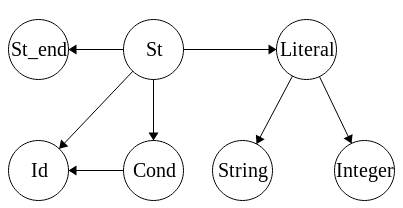
\includegraphics[scale=0.7, keepaspectratio]{Figures/strRegular_chap2_graph.png}
		\decoRule
	 	\caption[Graph of the strongly connected components of the example grammar]{The graph of the strongly connected components of the example grammar}
	 	\label{fig:chap2:strRegularGraph}
	\end{figure}
	\noindent The machine showed below is the machine generated from the \textit{Statement} non-terminal. As seen below all non-terminals that are not part of the same strongly connected component are viewed as terminals and put on arcs here. This is because there is certainty that this machine will not be reached again from within that machine such that infinite recursion could occur. This $DFA$ is a slightly more optimized version than what would have been obtained from following the described algorithm strictly. The other machine would have been larger, because naive powerset construction would embed the entire machine a second time due to the choice of the start state.
	\begin{figure}[H]
			\centering
			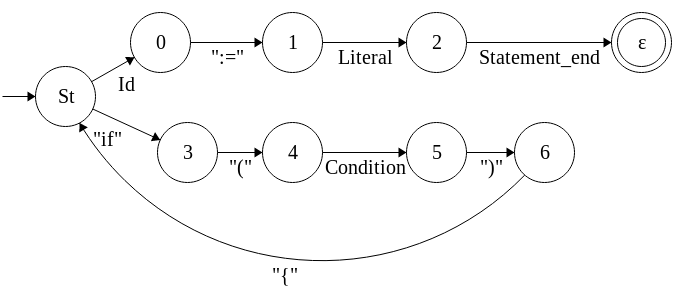
\includegraphics[width=\textwidth, keepaspectratio]{Figures/NFA_Statement_chap2.png}
			\decoRule
		 	\caption[DFA for Statement of the example grammar]{The DFA for the non-terminal Statement of the strongly regular grammar}
		 	\label{fig:chap2:NFA:Statement}
		\end{figure}
	
	\pagebreak
	
	\subsubsection{Conflict identification and resolution} \label{sec:ConflictResolutionAlgorithm}
	Now creating all these $DFA$'s helps with resolving much of the non-determinism for the syntax highlighter. However, there are still conflicts possible. As figure \ref{fig:ConflictExample} below shows, conflicts can still arise if a machine has an outgoing arc with a terminal and one with a non-terminal. If the corresponding machine of this non-terminal has the same terminal on an arc from its initial state then a choice conflict arises.\\\\
	The simplest fix for this is substituting the entire conflicting machine into the parent-machine. After this, rerun the $NFA2DFA$ algorithm. If conflicts remain, repeat. There are a number of functions needed in order to identify and fix the conflicts. Of which the most important ones are illustrated below. These functions ensure that conflicts are solved, however can take very long to complete. When working with smaller grammars, like DSL type of languages, these functions works fine. When working with larger grammars, where many conflicts arise, this process can take quite a while. The generated machines can also grow very large, in the order of tens of thousands states.\\\\
	To make this process more efficient, construct a tree-like structure of the connected components of the strongly regular version of the grammar. This is guaranteed to be a tree, because the connected components automatically join all cycles into one node, there can be multiple edges going into the same node though. Now use depth-first search from the start symbol's machine and resolve all conflicts in the leave nodes first and work upwards. This prevents having to solve the same conflict in the same machine multiple times.\\
	\begin{figure}[h]
\centering
\begin{center}
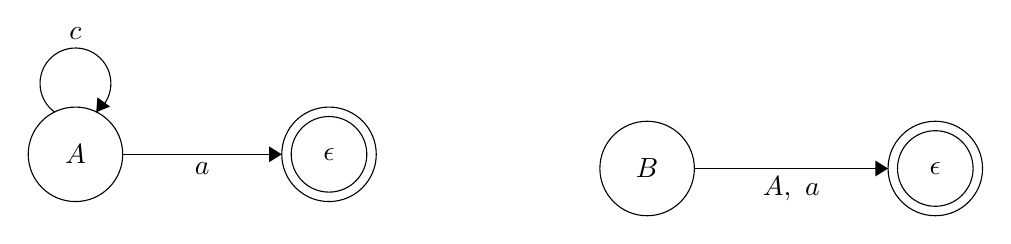
\begin{tikzpicture}[scale=0.2]
\tikzstyle{every node}+=[inner sep=0pt]
\draw [black] (11.2,-14.4) circle (3);
\draw (11.2,-14.4) node {$A$};
\draw [black] (47.5,-15.3) circle (3);
\draw (47.5,-15.3) node {$B$};
\draw [black] (65.8,-15.3) circle (3);
\draw (65.8,-15.3) node {$\epsilon$};
\draw [black] (65.8,-15.3) circle (2.4);
\draw [black] (27.3,-14.4) circle (3);
\draw (27.3,-14.4) node {$\epsilon$};
\draw [black] (27.3,-14.4) circle (2.4);
\draw [black] (9.877,-11.72) arc (234:-54:2.25);
\draw (11.2,-7.15) node [above] {$c$};
\fill [black] (12.52,-11.72) -- (13.4,-11.37) -- (12.59,-10.78);
\draw [black] (14.2,-14.4) -- (24.3,-14.4);
\fill [black] (24.3,-14.4) -- (23.5,-13.9) -- (23.5,-14.9);
\draw (19.25,-14.9) node [below] {$a$};
\draw [black] (50.5,-15.3) -- (62.8,-15.3);
\fill [black] (62.8,-15.3) -- (62,-14.8) -- (62,-15.8);
\draw (56.65,-15.8) node [below] {$A,\mbox{ }a$};
\end{tikzpicture}
\end{center}		
\decoRule
\caption[Conflicts in a graph]{Machine B has a conflict on encountering a terminal 'a'}
\label{fig:ConflictExample}
\end{figure}

	\pagebreak
	\subsubsection{Example}
	As the original example grammar did not contain any conflicts, the figure above will be used as an example. It shows two machines, one for the non-terminal $A$, and one for the non-terminal $B$. Now, for the output of the algorithms and functions below:\\
	\begin{align*}
	&alphabetOfState(A, M(A)) = \{a,\ c\}\\
	&alphabetOfState(\epsilon, M(A)) = \{\}\\
	&alphabetOfState(B, M(B)) = \{a,\ A\}\\
	&alphabetOfState(\epsilon, M(B)) = \{\}\\\\
	&firstTerminalOf(M(A), \{A, B\}, \{M(A), M(B)\}) = \{a, c\}\\
	&firstTerminalOf(M(B), \{A, B\}, \{M(A), M(B)\}) = \{a,\ c\ (from\ M(A))\, a\ (from\ M(A))\}\\\\
	&findConflicts(M(B), \{A, B\}, \{M(A), M(B)\}) = \{(B, A, \epsilon)\}\\
	&\qquad 1\ conflict\ in\ M(B)\ being:\ from\ B,\ taking\ A,\ to\ \epsilon\\
	&findConflicts(M(A), \{A, B\}, \{M(A), M(B)\}) = \{\}\\
	&\qquad 0\ conflicts\ in\ M(A)\\
	\end{align*}
	Below are the resulting machines shown that come from the algorithm. Left is the NFA obtained from only replacing the transition with the entire machine. Right is the DFA that is obtained from this NFA. With that, the DFA is the output of \textit{solveConflicts($M(B), \{M(B), M(A)\}, \{A, B\}, \{(B, A, \epsilon)\}$}).
	\begin{figure}[H]
		\centering
		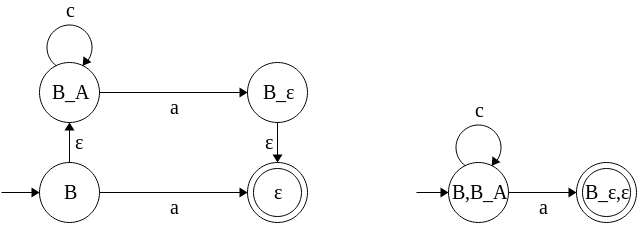
\includegraphics[width=\textwidth, keepaspectratio]{Figures/conflictSolvingChap2.png}
		\decoRule
	 	\caption[Conflict resolving NFA to DFA]{The NFA obtained from replacing the conflicting transition and the DFA obtained from the NFA.}
	 	\label{fig:chap2:NFA2DFA:ConflictSolving}
	\end{figure}
	
	
	\pagebreak
	\begin{algorithm}
	\caption{Resolve Conflicts}	\label{alg:conflicts}
	\begin{algorithmic}[1]
		\Function{solveConflicts}{dfa, allDfas, nonTerminals, conflicts}
		\ForAll {$\{tr | tr \in conflicts\}$}
			\State $nfa \gets replaceTransitionWithMachine(tr, dfa)$
		\EndFor
		\State $dfa \gets NFA2DFA(nfa)$
		\State $newConflicts \gets findConflicts(dfa, nonTerminals, allDfas)$
		\If {$newConflicts \not = \{\}$}
			\State \Return $solveConfcicts(dfa, allDfas, nonTerminals, newConflicts)$
		\Else	
			\State \Return $dfa$
		\EndIf
		\EndFunction
	\end{algorithmic}
\end{algorithm}
\vfill
\begin{algorithm}
	\caption{Find Conflicts}
	\begin{algorithmic}[1]		
		\Function{findConflicts}{dfa, nonTerminals, allDfas}
			\State $conflicts \gets \{\}$
			\ForAll {$\{state | state \in dfa.Q\}$}
				\State $tokens \gets alphabetOfState(state, dfa)$
				\State $ntsOfState \gets \{nt | nt \in tokens \land nt \in nonTerminals\}$
				\State $terminalsOfState \gets tokens - ntsOfState$
				\ForAll {$\{nt | nt \in ntsOfState\}$}
					\State $nextTerminals \gets firstTerminalOf(allDfas[nt], nonTerminals, allDfas)$
					\If {$(nextTerminals - terminalsOfState \not = \{\})$}
						\State $conflicts \gets conflicts + (state, nt, dfa.\delta(state, nt))$ 
					\EndIf
				\EndFor
			\EndFor
		\State \Return $conflicts$
		\EndFunction		
	\end{algorithmic}
\end{algorithm}
\vfill
\begin{algorithm}
	\caption{Get the terminals reachable from the first state of a machine}
	\begin{algorithmic}[1]		
		\Function{firstTerminalOf}{dfa, nonTerminals, allDfas}
			\State $tokens \gets alphabetOfState(dfa.q_0, dfa)$
			\State $terms \gets tokens - nonTerminals$
			\State $result \gets terms$
			\ForAll{$\{nt | nt \in (tokens - terms)\} $}
				\State $result \gets result + firstTerminalOf(allDfas[nt], nonTerminals, allDfas)$
			\EndFor		
			\State \Return $result$
		\EndFunction
	\end{algorithmic}
\end{algorithm}
	\pagebreak
	
	\subsection{Mapping machines to contexts}
	Once all non-terminals have their own conflictless machine it is possible to make a deterministic mapping from the machines to contexts and respective scopes. The general idea is to define a datatype corresponding to a state-based syntax highlighter. An algebraic datatype works very well because of the nested structures of a highlighter. Once the machines are translated into this datatype, define different methods on this datatype in order to write out highlighters for different editors. One general $SyntaxHighlighter$-datatype like this greatly improves on extensibility to new editors that use a similar structure. An alternative approach could be to define one $SyntaxHighlighter$-datatype per editor and write a specific machines-to-highlighter function per editor.\\\\
	The first of the aforementioned approaches is chosen and this translation step from machine to highlighter can be described as follows:
	\begin{enumerate}
	\item For each machine $M$ create a context $c_q$ per state $q \in M.Q$
	\item For each context $c_{q_1}$ add matches for each $tr=(q_1,\ a,\ q_2) \Rightarrow q_1, q_2 \in Q \land a \in \Sigma$:
		\subitem $c_{q_1}.matches$ += $(a,\ null(),\ set(c_{q_2}))$
	\item For context $c_{q_1}$ add matches for each $tr=(q_1, A, q_2) \Rightarrow q_1, q_2 \in Q \land A \in V$:
		\subitem $tokens = firstTerminalsOf(M(A))$
		\subitem $c_{q_1}.matches$ += $(lookahead(any(tokens)),\ null(),\ set([c_{q_2},\ c_{A.q_0}]))$\vspace{0.05in}\\
		The regular expression is supposed to be a lookahead match on any of the terminals of the machine $M(A)$. This is needed because lookahead does not consume the actual pattern that was matched. This will be done by the first context of $M(A)$. The action replaces the old context $c_{q_1}$ with the $c_{q_2}$ and pushes the first context of machine $M(A)$ called $c_{A.{q_0}}$ on top of that. So the highlighter is now in machine $M(A)$ and once this pops itself off, it ends up in the next state of the original machine. 
	\item For each context $c_{A.q} \Rightarrow q \in M(A).F$ take one of the action described in the next section (\nameref{sec:FinalStateCases}).
	\item For the start symbol $S$ create a context $c_{main} = include(c_{S.{q_0}})$
		\subitem Creates an empty $main$ context that includes the first actual context.
		\subitem $H.main = c_{main}$
	\item Identify all matches that need to have a scope assigned and do so. This can be done based on the information gathered in \ref{sec:Pipeline}. For giving entire machines a scope you need to assign the scope to all matches of all contexts corresponding with this machine.
	\item Remove all contexts that are unreachable
	\end{enumerate}
	
	\pagebreak
	
	\subsubsection{Final State Cases} \label{sec:FinalStateCases}	
	There are two cases for a final state of a machine. The state is either final with no outgoing arcs (I.E. a \textit{sink-state}). Or it still has other outgoing arcs (\textit{non-sink state}). These cases could be treated differently when mapping them to contexts.
	\begin{itemize}
		\item \emph{\textbf{Sink-states:}}\\
		For each sink-state there will be no match created (yet), because it has no outgoing arcs. The only thing to be added is a match that pops this context and machine off of the stack.\\
		Let a final sink-state be $q_{fs}$ then:
			\subitem $c_{q_{fs}}.matches$ += $(\epsilon,\ null(),\ pop())$\vspace{0.05in}\\
			This just matches the empty regex, this always succeeds, and then pops. A different approach would be to choose, in the last match that would lead to $c_{q_{fs}}$, to $pop()$ here and to not $push()$ nor $set()$ this context in the first place. In terms of the above sketch:
			\subitem For each $c_{q_1} \in C$, for each $tr:(q_1,\ a,\ q_{fs}) \Rightarrow q_1, q_{fs} \in Q \land a \in \Sigma$
				\subsubitem $\quad c_{q_1}.matches$ += $(a,\ null(),\ pop())$
			\subitem For each $c_{q_1} \in C$, for each $tr:(q_1, A, q_2) \Rightarrow q_1, q_{fs} \in Q \land A \in V$
				\subsubitem $\quad tokens = firstTerminalsOf(M(A))$
				\subsubitem $\quad c_{q_1}.matches$ += $(lookahead(any(tokens)),\ null(),\ set(c_{A.q_0}))$
		\item \emph{\textbf{Non-Sink states:}}\\
		These states are harder to reason about. There are choices that need to be made, which is hard to do in a deterministic way. A state like this means that you can either \emph{pop} the current machine, or continue consuming with this machine. There could be conflicts here again as well, for example:
		\subitem The current machine is $B$.
		\subitem A final non-sink state $A.q_f \in F$ has 1 transition: $tr=(q_f,\ a,\ q_f)\ :\ a \in A.\Sigma$
		\subitem The state $B.q_x$ has a transition: $tr=(q_x,\ a,\ q_y)\ :\ a \in B.\Sigma$			
		\subitem The context stack looks like this: $[c_{B.q_x},\ c_{A.q_f}]$
		\subitem This is a conflict, do you pop and consume $a$, or continue and consume $a$?
		\subitem There is a choice to be made:
			\subsubitem 1. Resolve these end-of-machine conflicts
			\subsubitem 2. Always pick the $pop$-action
			\subsubitem 3. Always pick the $continue$-action
		\subitem Highlighters do not need to be perfect, so for now pick option 3.
		\subitem To accomplish this, add the same match as if this were a \textit{sink-state}.
		\subitem This has to be the final match, or the other matches become unreachable.
	\end{itemize}
	\pagebreak
	
	\subsubsection{Example}
	Below is a stepwise example of the just described mapping of the machine shown in figure \ref{fig:chap2:NFA:Statement}. For ease of reading it is written in Sublime Syntax format.
\begin{enumerate}
\item For each machine $M$ create a context $c_q$ per state $q \in M.Q$
\begin{lstlisting}[language=SublimeSyntax]
Statement_St:
Statement_0:
Statement_1:
Statement_2:
Statement_3:
Statement_4:
Statement_5:
Statement_6:
Statement_epsilon:
\end{lstlisting}
\item For each context $c_{q_1}$ add matches for each $tr=(q_1,\ a,\ q_2) \Rightarrow q_1, q_2 \in Q \land a \in \Sigma$:
\begin{lstlisting}[language=SublimeSyntax]
Statement_St:
	- match: 'if'
	  set: [Statement_3]
Statement_0:
	- match: ':='
	  set: [Statement_1]
Statement_1:
Statement_2:
Statement_3:
	- match: '('
	  set: [Statement_4]
Statement_4:
Statement_5:
	- match: ')'
	  set: [Statement_6]
Statement_6:
	- match: '{'
	  set: [Statement_St]
Statement_epsilon:
\end{lstlisting}	
\item For context $c_{q_1}$ add matches for each $tr=(q_1, A, q_2) \Rightarrow q_1, q_2 \in Q \land A \in V$:
\begin{lstlisting}[language=SublimeSyntax]
Statement_Start:
	- match: 'if'
	  set: [Statement_3]
 	- match: '?=([a-z]+)'
	  set: [Statement_0, Id_Start]
Statement_0:
	- match: ':='
	  set: [Statement_1]
Statement_1:
 	- match: '?=(\"|[0-9]+)'
	  set: [Statement_2, Literal_Start]
	  
Statement_2:
 	- match: '?=((}| ))'
	  set: [Statement_epsilon, Statement_end_Start]
Statement_3:
	- match: '('
	  set: [Statement_4]
Statement_4:
 	- match: '?=([a-z]+)'
	  set: [Statement_5, Condition_Start]
Statement_5:
	- match: ')'
	  set: [Statement_6]
Statement_6:
	- match: '{'
	  set: [Statement_Start]
Statement_epsilon:
\end{lstlisting}
\item For each context $c_{A.q} \Rightarrow q \in M(A).F$ take one of the action described in \nameref{sec:FinalStateCases}.
\begin{lstlisting}[language=SublimeSyntax]
Statement_epsilon:
	- match: ''
	  pop: true
\end{lstlisting}
\item For the start symbol $S$ create a context $c_{main} = include(c_{S.{q_0}})$
\begin{lstlisting}[language=SublimeSyntax]
main:
	- include: Statement_Start
\end{lstlisting}
\item Identify all matches that need to have a scope assigned and do so. This can be done based on the information gathered in \ref{sec:Pipeline}. For giving entire machines a scope you need to assign the scope to all matches of all contexts corresponding with this machine.
\begin{lstlisting}[language=SublimeSyntax]
Statement_Start:
	- match: 'if'
	  scope: keyword.control.flow
	  set: [Statement_3]
 	- match: '?=([a-z]+)'
	  set: [Statement_0, Id_Start]
\end{lstlisting}
\item Remove all contexts that are unreachable\\
-
\end{enumerate}
		